\documentclass[tikz,border=12pt]{standalone}
\usepackage{amsmath}
\begin{document}
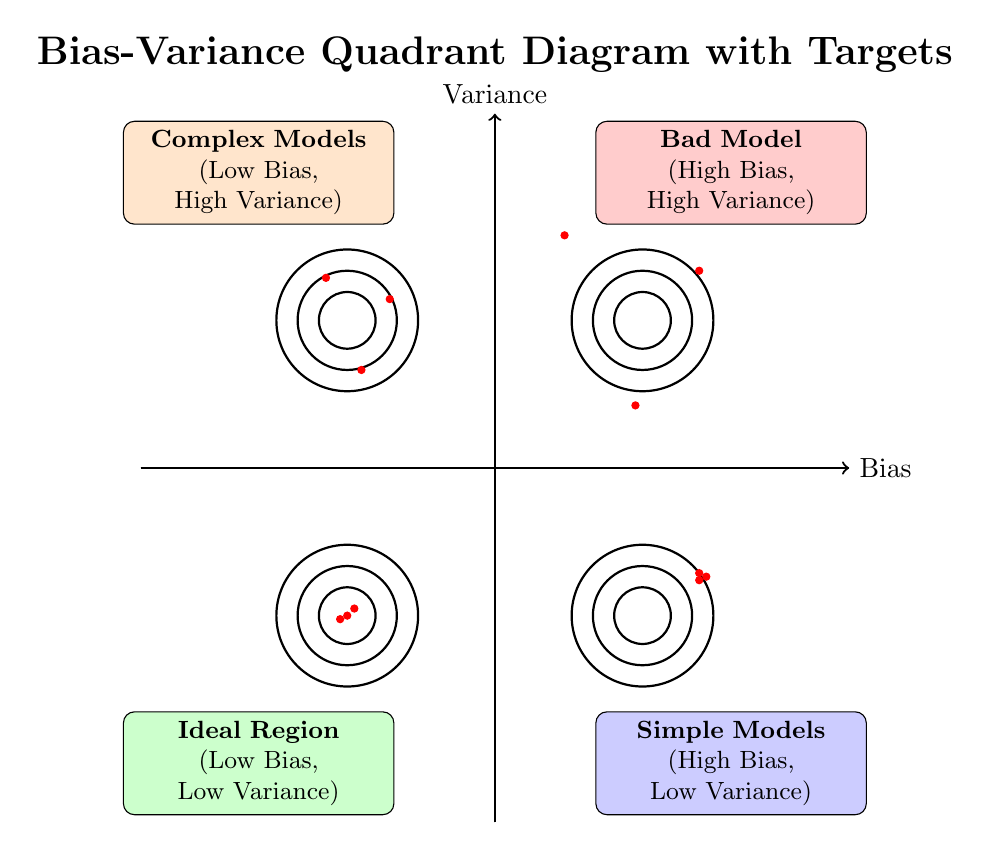
\begin{tikzpicture}[scale=1.5, every node/.style={font=\small}]

  %%%%%%%%%%%%%%%%%%%%%%%%%%%%%%
  % Draw the bias-variance axes %
  %%%%%%%%%%%%%%%%%%%%%%%%%%%%%%
  \draw[->, thick] (-3,0) -- (3,0) node[right, font=\normalsize] {Bias};
  \draw[->, thick] (0,-3) -- (0,3) node[above, font=\normalsize] {Variance};
  \draw[dashed] (-3,0) -- (3,0);
  \draw[dashed] (0,-3) -- (0,3);

  %%%%%%%%%%%%%%%%%%%%%%%%%%%%%%
  % Add quadrant labels/boxes  %
  %%%%%%%%%%%%%%%%%%%%%%%%%%%%%%
  % Bottom Right: High Bias, Low Variance (Simple Models)
  \node[draw, rounded corners, fill=blue!20, align=center, text width=3.2cm] at (2,-2.5)
        {\textbf{Simple Models}\\(High Bias, Low Variance)};
  % Top Left: Low Bias, High Variance (Complex Models)
  \node[draw, rounded corners, fill=orange!20, align=center, text width=3.2cm] at (-2,2.5)
        {\textbf{Complex Models}\\(Low Bias, High Variance)};
  % Bottom Left: Ideal Region (Low Bias, Low Variance)
  \node[draw, rounded corners, fill=green!20, align=center, text width=3.2cm] at (-2,-2.5)
        {\textbf{Ideal Region}\\(Low Bias, Low Variance)};
  % Top Right: High Bias, High Variance
  \node[draw, rounded corners, fill=red!20, align=center, text width=3.2cm] at (2,2.5)
        {\textbf{Bad Model}\\(High Bias, High Variance)};

  %%%%%%%%%%%%%%%%%%%%%%%%%%%%%%
  % Combined diagram title     %
  %%%%%%%%%%%%%%%%%%%%%%%%%%%%%%
  \node at (0,3.5) {\Large \textbf{Bias-Variance Quadrant Diagram with Targets}};

  %%%%%%%%%%%%%%%%%%%%%%%%%%%%%%%%%%%%%%%%%%%%%%%%%%%%%%%%%%%%%%%%%%%%%%%
  % Now overlay the target diagrams into each quadrant using scopes.   %
  % Each target diagram is scaled (here scale=0.6) and shifted so its center %
  % coincides with the quadrant's center.                                %
  %%%%%%%%%%%%%%%%%%%%%%%%%%%%%%%%%%%%%%%%%%%%%%%%%%%%%%%%%%%%%%%%%%%%%%%

  % Low Bias, Low Variance Target (Ideal Region: bottom-left quadrant)
  \begin{scope}[shift={(-1.25,-1.25)}, scale=0.6]
    \draw[thick] (0,0) circle (1.0);
    \draw[thick] (0,0) circle (0.7);
    \draw[thick] (0,0) circle (0.4);
    % Darts clustered near center
    \filldraw[red] (0,0) circle (0.05);
    \filldraw[red] (0.1,0.1) circle (0.05);
    \filldraw[red] (-0.1,-0.05) circle (0.05);
  \end{scope}

  % High Bias, Low Variance Target (Simple Models: bottom-right quadrant)
  \begin{scope}[shift={(1.25,-1.25)}, scale=0.6]
    \draw[thick] (0,0) circle (1.0);
    \draw[thick] (0,0) circle (0.7);
    \draw[thick] (0,0) circle (0.4);
    % Darts clustered but off-center
    \filldraw[red] (0.8,0.5) circle (0.05);
    \filldraw[red] (0.8,0.6) circle (0.05);
    \filldraw[red] (0.9,0.55) circle (0.05);
  \end{scope}

  % Low Bias, High Variance Target (Complex Models: top-left quadrant)
  \begin{scope}[shift={(-1.25,1.25)}, scale=0.6]
    \draw[thick] (0,0) circle (1.0);
    \draw[thick] (0,0) circle (0.7);
    \draw[thick] (0,0) circle (0.4);
    % Darts scattered but averaging near center
    \filldraw[red] (0.6,0.3) circle (0.05);
    \filldraw[red] (-0.3,0.6) circle (0.05);
    \filldraw[red] (0.2,-0.7) circle (0.05);
  \end{scope}

  % High Bias, High Variance Target (top-right quadrant)
  \begin{scope}[shift={(1.25,1.25)}, scale=0.6]
    \draw[thick] (0,0) circle (1.0);
    \draw[thick] (0,0) circle (0.7);
    \draw[thick] (0,0) circle (0.4);
    % Darts scattered with off-center average
    \filldraw[red] (-1.1,1.2) circle (0.05);
    \filldraw[red] (0.8,0.7) circle (0.05);
    \filldraw[red] (-0.1,-1.2) circle (0.05);
  \end{scope}

\end{tikzpicture}
\end{document}
